\documentclass[11pt,a4paper]{article}
\usepackage{graphicx}
\usepackage{tcolorbox}
\usepackage{xcolor}
\usepackage{geometry}
\usepackage{tikz}
\geometry{margin=0.8in}

% Define colors
\definecolor{mlblue}{RGB}{31, 119, 180}
\definecolor{mlorange}{RGB}{255, 127, 14}
\definecolor{mlgreen}{RGB}{44, 160, 44}
\definecolor{mlred}{RGB}{214, 39, 40}
\definecolor{mlpurple}{RGB}{148, 103, 189}
\definecolor{mlyellow}{RGB}{241, 196, 15}

\title{\Large\textbf{Discovery 5: The Goldilocks Problem}\\
\vspace{0.3em}
\normalsize Not Too Few, Not Too Many, Just Right}
\date{}

\begin{document}
\maketitle
\vspace{-2em}

\section*{Same Data, Different Stories}

\begin{center}
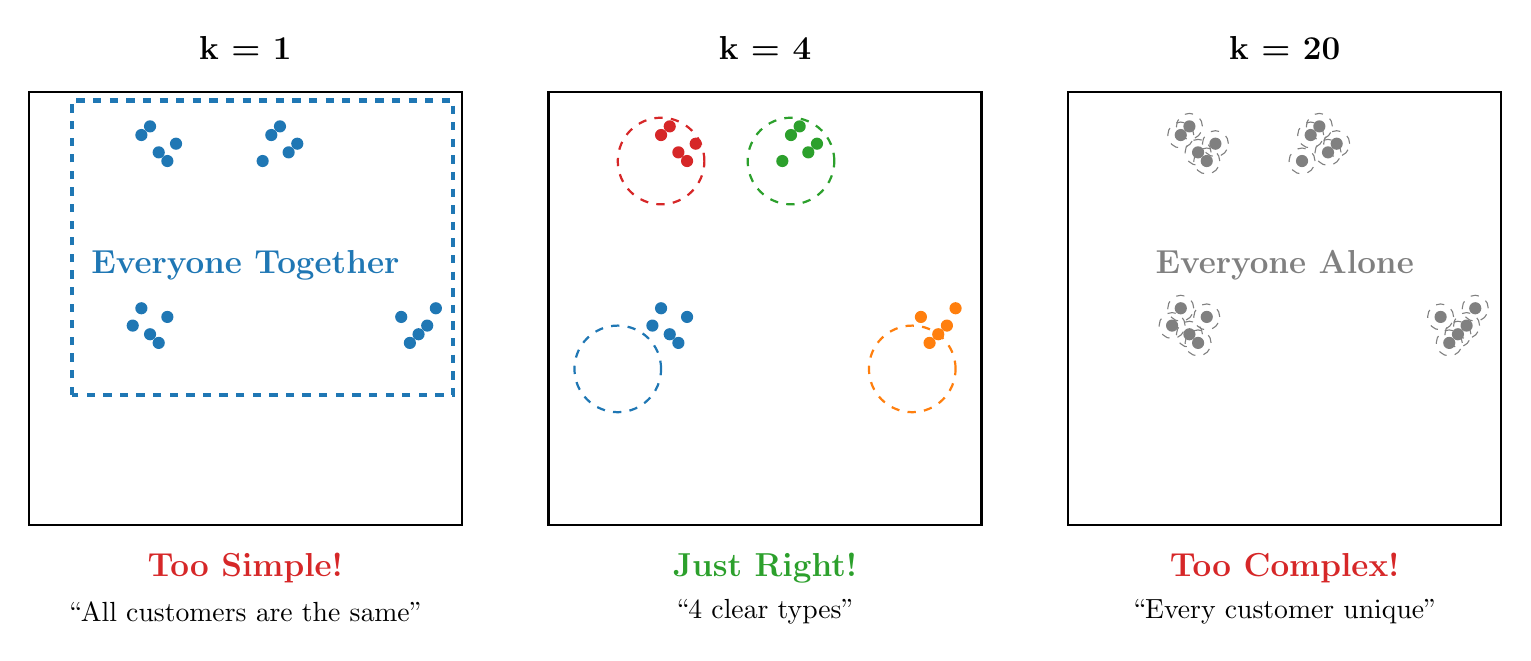
\begin{tikzpicture}[scale=1.1]
% Generate same data points for all three
\def\datapoints{
    (1.2,2.3), (1.5,2.1), (1.3,2.5), (1.6,2.4), (1.4,2.2),
    (4.5,2.2), (4.3,2.4), (4.6,2.3), (4.4,2.1), (4.7,2.5),
    (2.8,4.5), (3,4.3), (2.9,4.6), (3.1,4.4), (2.7,4.2),
    (1.5,4.3), (1.3,4.5), (1.6,4.2), (1.4,4.6), (1.7,4.4)
}

% k=1: Everything together
\begin{scope}[shift={(0,0)}]
\draw[thick] (0,0) rectangle (5,5);
\node[font=\large\bfseries] at (2.5,5.5) {k = 1};
\node[font=\large\bfseries, mlred] at (2.5,-0.5) {Too Simple!};
\draw[mlblue, ultra thick, dashed] (0.5,1.5) rectangle (4.9,4.9);
\foreach \point in \datapoints {
    \fill[mlblue] \point circle (2pt);
}
\node[mlblue, font=\large] at (2.5,3) {\textbf{Everyone Together}};
\node at (2.5,-1) {``All customers are the same''};
\end{scope}

% k=4: Just right
\begin{scope}[shift={(6,0)}]
\draw[thick] (0,0) rectangle (5,5);
\node[font=\large\bfseries] at (2.5,5.5) {k = 4};
\node[font=\large\bfseries, mlgreen] at (2.5,-0.5) {Just Right!};
% Draw 4 distinct clusters
\draw[mlblue, thick, dashed] (0.8,1.8) circle (0.5);
\draw[mlorange, thick, dashed] (4.2,1.8) circle (0.5);
\draw[mlgreen, thick, dashed] (2.8,4.2) circle (0.5);
\draw[mlred, thick, dashed] (1.3,4.2) circle (0.5);
\foreach \point in {(1.2,2.3), (1.5,2.1), (1.3,2.5), (1.6,2.4), (1.4,2.2)} {
    \fill[mlblue] \point circle (2pt);
}
\foreach \point in {(4.5,2.2), (4.3,2.4), (4.6,2.3), (4.4,2.1), (4.7,2.5)} {
    \fill[mlorange] \point circle (2pt);
}
\foreach \point in {(2.8,4.5), (3,4.3), (2.9,4.6), (3.1,4.4), (2.7,4.2)} {
    \fill[mlgreen] \point circle (2pt);
}
\foreach \point in {(1.5,4.3), (1.3,4.5), (1.6,4.2), (1.4,4.6), (1.7,4.4)} {
    \fill[mlred] \point circle (2pt);
}
\node at (2.5,-1) {``4 clear types''};
\end{scope}

% k=20: Every point alone
\begin{scope}[shift={(12,0)}]
\draw[thick] (0,0) rectangle (5,5);
\node[font=\large\bfseries] at (2.5,5.5) {k = 20};
\node[font=\large\bfseries, mlred] at (2.5,-0.5) {Too Complex!};
\foreach \point in \datapoints {
    \fill[gray] \point circle (2pt);
    \draw[gray, dashed] \point circle (0.15);
}
\node[gray, font=\large] at (2.5,3) {\textbf{Everyone Alone}};
\node at (2.5,-1) {``Every customer unique''};
\end{scope}
\end{tikzpicture}
\end{center}

\vspace{1em}

\begin{tcolorbox}[colback=mlyellow!20, colframe=mlyellow!70]
\centering\Large
\textbf{How many groups do YOU see?}
\end{tcolorbox}

\vspace{2em}

\section*{The Elbow Test}

\begin{center}
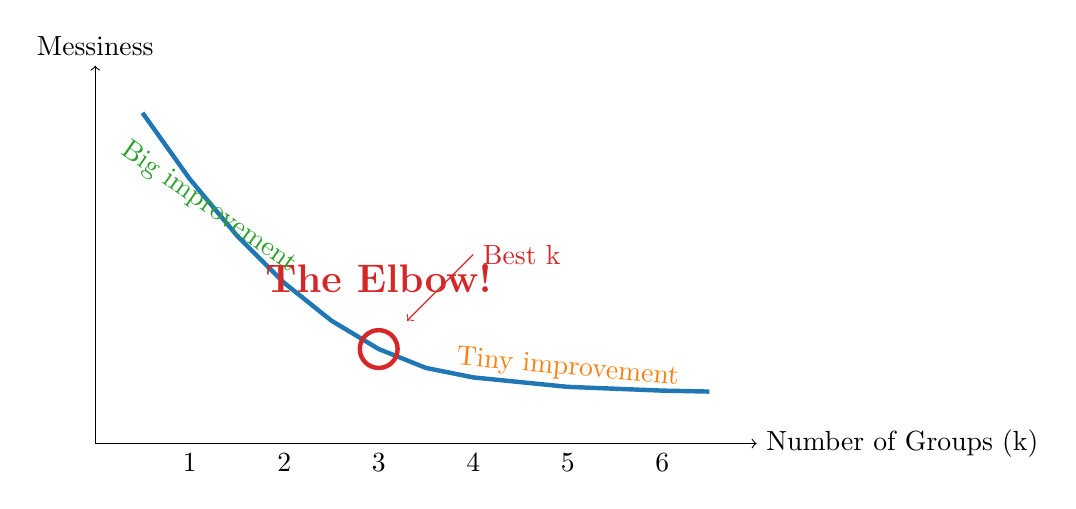
\begin{tikzpicture}[scale=1.2]
\draw[->] (0,0) -- (7,0) node[right] {Number of Groups (k)};
\draw[->] (0,0) -- (0,4) node[above] {Messiness};

% Draw the elbow curve
\draw[ultra thick, mlblue] plot coordinates {(0.5,3.5) (1,2.8) (1.5,2.2) (2,1.7) (2.5,1.3) (3,1) (3.5,0.8) (4,0.7) (4.5,0.65) (5,0.6) (5.5,0.58) (6,0.56) (6.5,0.55)};

% Mark the elbow
\draw[mlred, ultra thick] (3,1) circle (0.2);
\node[mlred, above] at (3,1.5) {\Large\textbf{The Elbow!}};
\draw[mlred, <-] (3.3,1.3) -- (4,2) node[right] {Best k};

% Labels
\foreach \x in {1,2,3,4,5,6} {
    \node[below] at (\x,0) {\x};
}

% Annotations
\node[mlgreen, rotate=-35] at (1.2,2.5) {Big improvement};
\node[mlorange, rotate=-5] at (5,0.8) {Tiny improvement};
\end{tikzpicture}
\end{center}

\newpage

\section*{Try It: Pizza Toppings}

\begin{center}
\Large\textbf{20 pizzas ordered last week. How many types?}

\vspace{1em}

\begin{tikzpicture}[scale=0.8]
% Draw 20 pizza circles randomly
\foreach \i in {1,...,20} {
    \pgfmathsetmacro{\x}{rand*10}
    \pgfmathsetmacro{\y}{rand*6}
    \draw[thick] (\x,\y) circle (0.4);
    \pgfmathtruncatemacro{\topping}{random(0,4)}
    \ifnum\topping=0
        \fill[mlred] (\x,\y) ++(0.1,0.1) circle (0.05);
        \fill[mlred] (\x,\y) ++(-0.1,0.1) circle (0.05);
        \fill[mlred] (\x,\y) ++(0,-0.1) circle (0.05);
    \fi
    \ifnum\topping=1
        \fill[mlorange] (\x,\y) ++(-0.15,0) rectangle ++(0.3,0.05);
        \fill[mlorange] (\x,\y) ++(0,-0.15) rectangle ++(0.05,0.3);
    \fi
    \ifnum\topping=2
        \fill[mlgreen] (\x,\y) ++(0.1,0.05) circle (0.03);
        \fill[mlgreen] (\x,\y) ++(-0.1,0.05) circle (0.03);
        \fill[mlgreen] (\x,\y) ++(0.05,-0.1) circle (0.03);
        \fill[mlgreen] (\x,\y) ++(-0.05,-0.1) circle (0.03);
    \fi
    \ifnum\topping=3
        \fill[mlpurple] (\x,\y) circle (0.15);
    \fi
    \ifnum\topping=4
        \draw[mlblue, thick] (\x,\y) ++(0.1,0.1) -- ++(-0.2,-0.2);
        \draw[mlblue, thick] (\x,\y) ++(-0.1,0.1) -- ++(0.2,-0.2);
    \fi
}
\end{tikzpicture}

\vspace{1em}

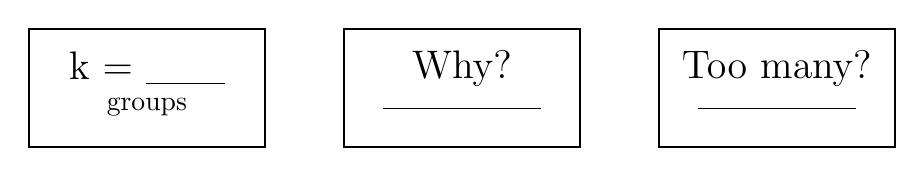
\begin{tikzpicture}[scale=1]
\draw[thick] (0,0) rectangle (3,1.5);
\node at (1.5,1) {\Large k = \underline{\hspace{1cm}}};
\node at (1.5,0.5) {groups};

\draw[thick] (4,0) rectangle (7,1.5);
\node at (5.5,1) {\Large Why?};
\node at (5.5,0.5) {\underline{\hspace{2cm}}};

\draw[thick] (8,0) rectangle (11,1.5);
\node at (9.5,1) {\Large Too many?};
\node at (9.5,0.5) {\underline{\hspace{2cm}}};
\end{tikzpicture}
\end{center}

\vspace{2em}

\section*{Real World Goldilocks}

\begin{center}
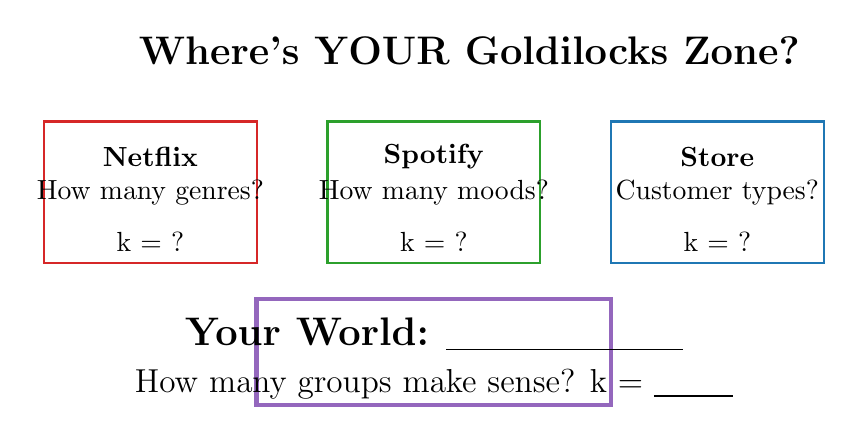
\begin{tikzpicture}[scale=0.9]
\node[font=\Large\bfseries] at (6,5) {Where's YOUR Goldilocks Zone?};

% Netflix genres
\draw[thick, mlred] (0,2) rectangle (3,4);
\node at (1.5,3.5) {\textbf{Netflix}};
\node at (1.5,3) {How many genres?};
\node at (1.5,2.3) {k = ?};

% Spotify moods
\draw[thick, mlgreen] (4,2) rectangle (7,4);
\node at (5.5,3.5) {\textbf{Spotify}};
\node at (5.5,3) {How many moods?};
\node at (5.5,2.3) {k = ?};

% Customer types
\draw[thick, mlblue] (8,2) rectangle (11,4);
\node at (9.5,3.5) {\textbf{Store}};
\node at (9.5,3) {Customer types?};
\node at (9.5,2.3) {k = ?};

% Your choice
\draw[ultra thick, mlpurple] (3,0) rectangle (8,1.5);
\node at (5.5,1) {\Large\textbf{Your World:} \underline{\hspace{3cm}}};
\node at (5.5,0.3) {\large How many groups make sense? k = \underline{\hspace{1cm}}};
\end{tikzpicture}
\end{center}

\vspace{1em}

\begin{tcolorbox}[colback=mlpurple!10, colframe=mlpurple!50]
\centering\large
\textbf{Next Class:} How ML finds the perfect k automatically
\end{tcolorbox}

\end{document}